
\subsection{Bias Variance Trade-off}

\begin{frame}[t]
    \frametitle{Bias Variance Trade-off}
    \framesubtitle{The Expected Generalization Error}
    \onslide<1->{
            $y = f(x) + \epsilon$ and 
            $\epsilon \sim \mathcal{N}(0,\sigma_{\epsilon}^2)$\\
            \smallbreak
            Estimate of $f(x)$:$\quad \hat{f}(x)$\\
            \smallbreak
            The expected generalization error: $\boldsymbol{Err}(\hat{f}(x))$ \\
    }
    \bigbreak
    \onslide<2->{
        The decomposition of a model's expected generalization error is
        \begin{block}{}
            \begin{center}
                $\boldsymbol{Err}(\hat{f}(x)) = \sigma_{\epsilon}^2 + [Bias(\hat{f}(x))]^2 + Var(\hat{f}(x))$
            \end{center}
        \end{block}
    }
    \bigbreak
    \onslide<3->{
        \quad $\sigma_{\epsilon}^2$ is irreducible and independent of the model. \\
        \bigbreak
        \quad Trade-off between bias and variance. \\
        \smallbreak
        \quad \textbf{Aim:} Decrease variance while keeping bias unincreased.
        }
\end{frame}

\begin{frame}
    \frametitle{Bias-Variance Trade-off}
    \framesubtitle{Illustration}
    \begin{figure}      
        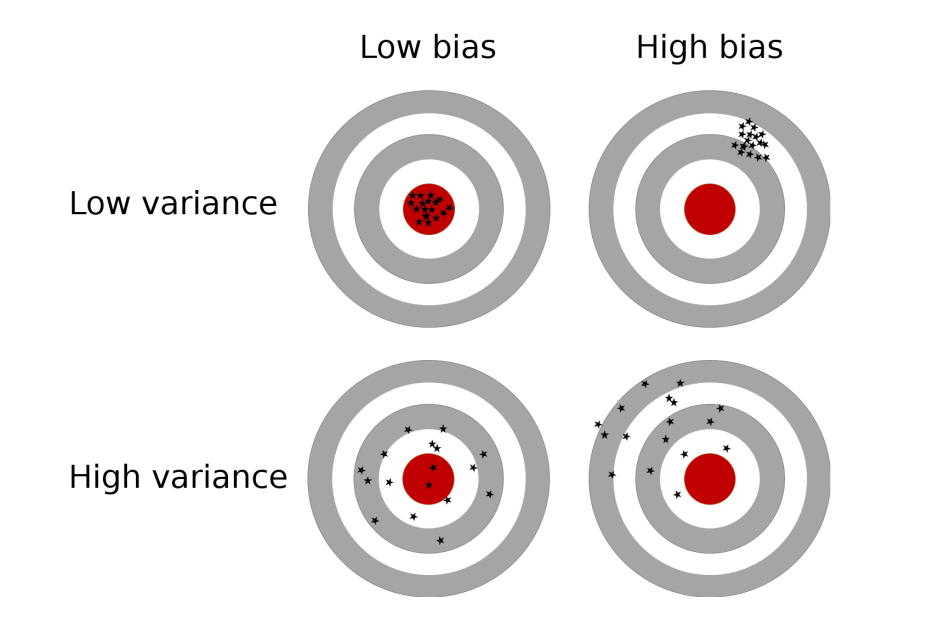
\includegraphics[height=0.6\textheight]{images/bias-variance.png}
    \end{figure}
    \begin{center}
    Decision trees generally have low bias and high variance.
    \end{center}
\end{frame}

    %\begin{columns}[c] % The "c" option specifies centered vertical alignment while the "t" option is used for top vertical alignment
    
    %\column{.45\textwidth} % Left column and width
    %\textbf{Heading}
    %\begin{enumerate}
    %\item Statement
    %\item Explanation
    %\item Example
    %\end{enumerate}
    
    %\column{.5\textwidth} % Right column and width
    %Lorem ipsum dolor sit amet, consectetur adipiscing elit. Integer lectus nisl, ultricies in feugiat rutrum, porttitor sit amet augue. Aliquam ut tortor mauris. Sed volutpat ante purus, quis accumsan dolor.
    
    %\end{columns}
